% !TEX encoding = UTF-8 Unicode
\documentclass[10pt]{standalone}\usepackage{tikz,graphicx}
\usepackage{fontspec}
\setmainfont{Arial}
\setsansfont{Arial}\begin{document}

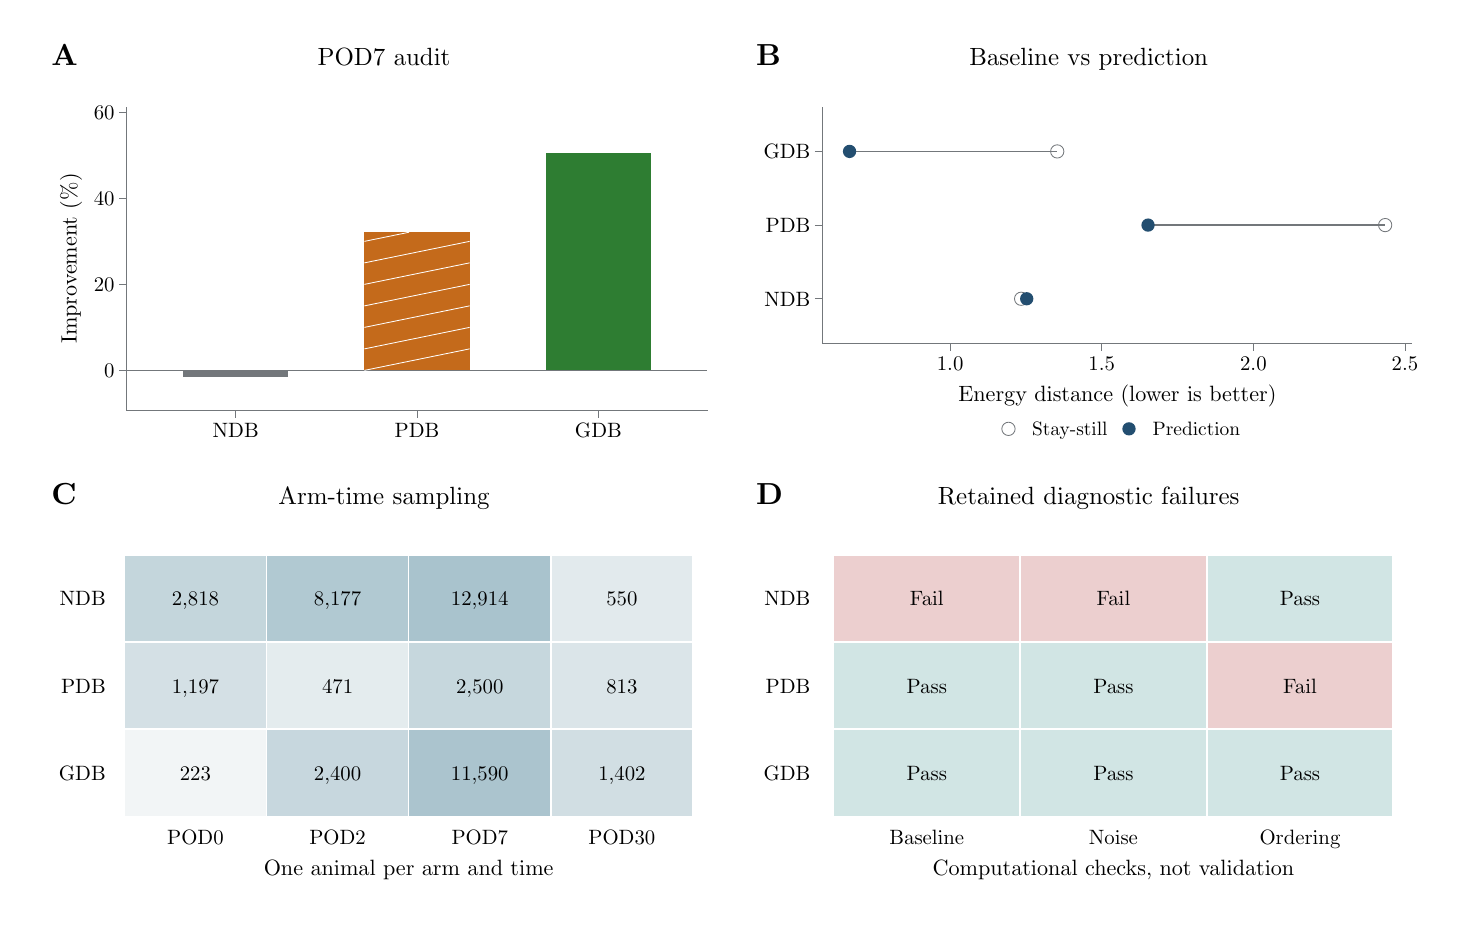
\begin{tikzpicture}[x=1pt,y=1pt]
\definecolor{fillColor}{RGB}{255,255,255}
\path[use as bounding box,fill=fillColor,fill opacity=0.00] (0,0) rectangle (512.15,315.83);
\begin{scope}
\path[clip] (  0.00,  0.00) rectangle (512.15,315.83);
\definecolor{drawColor}{RGB}{0,0,0}

\node[text=drawColor,anchor=base west,inner sep=0pt, outer sep=0pt, scale=  1.10] at (  8.54,302.26) {\bfseries A};

\node[text=drawColor,anchor=base,inner sep=0pt, outer sep=0pt, scale=  0.90] at (128.75,302.27) {POD7 audit};
\end{scope}
\begin{scope}
\path[clip] (  8.54,162.89) rectangle (248.96,292.21);
\definecolor{fillColor}{RGB}{255,255,255}

\path[fill=fillColor] (  8.54,162.89) rectangle (248.96,292.21);
\end{scope}
\begin{scope}
\path[clip] ( 35.85,177.70) rectangle (245.55,287.09);
\definecolor{fillColor}{RGB}{255,255,255}

\path[fill=fillColor] ( 35.85,177.70) rectangle (245.55,287.09);
\definecolor{fillColor}{RGB}{115,119,123}

\path[fill=fillColor] ( 56.16,189.68) rectangle ( 94.17,191.99);
\definecolor{fillColor}{RGB}{196,106,27}

\path[fill=fillColor] (121.69,191.99) rectangle (159.70,241.90);
\definecolor{fillColor}{RGB}{46,125,50}

\path[fill=fillColor] (187.22,191.99) rectangle (225.23,270.65);
\definecolor{drawColor}{RGB}{115,119,123}

\path[draw=drawColor,line width= 0.3pt,line join=round] ( 35.85,191.99) -- (245.55,191.99);
\definecolor{drawColor}{RGB}{255,255,255}

\path[draw=drawColor,line width= 0.3pt,line join=round] (121.69,191.99) -- (159.70,199.76);

\path[draw=drawColor,line width= 0.3pt,line join=round] (121.69,199.76) -- (159.70,207.53);

\path[draw=drawColor,line width= 0.3pt,line join=round] (121.69,207.53) -- (159.70,215.30);

\path[draw=drawColor,line width= 0.3pt,line join=round] (121.69,215.30) -- (159.70,223.07);

\path[draw=drawColor,line width= 0.3pt,line join=round] (121.69,223.07) -- (159.70,230.84);

\path[draw=drawColor,line width= 0.3pt,line join=round] (121.69,230.84) -- (159.70,238.61);

\path[draw=drawColor,line width= 0.3pt,line join=round] (121.69,238.61) -- (137.80,241.90);
\end{scope}
\begin{scope}
\path[clip] (  0.00,  0.00) rectangle (512.15,315.83);
\definecolor{drawColor}{RGB}{115,119,123}

\path[draw=drawColor,line width= 0.3pt,line join=round,line cap=rect] ( 35.85,177.70) --
	( 35.85,287.09);
\end{scope}
\begin{scope}
\path[clip] (  0.00,  0.00) rectangle (512.15,315.83);
\definecolor{drawColor}{RGB}{0,0,0}

\node[text=drawColor,anchor=base east,inner sep=0pt, outer sep=0pt, scale=  0.75] at ( 31.40,189.31) {0};

\node[text=drawColor,anchor=base east,inner sep=0pt, outer sep=0pt, scale=  0.75] at ( 31.40,220.39) {20};

\node[text=drawColor,anchor=base east,inner sep=0pt, outer sep=0pt, scale=  0.75] at ( 31.40,251.46) {40};

\node[text=drawColor,anchor=base east,inner sep=0pt, outer sep=0pt, scale=  0.75] at ( 31.40,282.54) {60};
\end{scope}
\begin{scope}
\path[clip] (  0.00,  0.00) rectangle (512.15,315.83);
\definecolor{drawColor}{RGB}{115,119,123}

\path[draw=drawColor,line width= 0.3pt,line join=round] ( 33.00,191.99) --
	( 35.85,191.99);

\path[draw=drawColor,line width= 0.3pt,line join=round] ( 33.00,223.07) --
	( 35.85,223.07);

\path[draw=drawColor,line width= 0.3pt,line join=round] ( 33.00,254.15) --
	( 35.85,254.15);

\path[draw=drawColor,line width= 0.3pt,line join=round] ( 33.00,285.22) --
	( 35.85,285.22);
\end{scope}
\begin{scope}
\path[clip] (  0.00,  0.00) rectangle (512.15,315.83);
\definecolor{drawColor}{RGB}{115,119,123}

\path[draw=drawColor,line width= 0.3pt,line join=round,line cap=rect] ( 35.85,177.70) --
	(245.55,177.70);
\end{scope}
\begin{scope}
\path[clip] (  0.00,  0.00) rectangle (512.15,315.83);
\definecolor{drawColor}{RGB}{115,119,123}

\path[draw=drawColor,line width= 0.3pt,line join=round] ( 75.17,174.85) --
	( 75.17,177.70);

\path[draw=drawColor,line width= 0.3pt,line join=round] (140.70,174.85) --
	(140.70,177.70);

\path[draw=drawColor,line width= 0.3pt,line join=round] (206.23,174.85) --
	(206.23,177.70);
\end{scope}
\begin{scope}
\path[clip] (  0.00,  0.00) rectangle (512.15,315.83);
\definecolor{drawColor}{RGB}{0,0,0}

\node[text=drawColor,anchor=base,inner sep=0pt, outer sep=0pt, scale=  0.75] at ( 75.17,167.88) {NDB};

\node[text=drawColor,anchor=base,inner sep=0pt, outer sep=0pt, scale=  0.75] at (140.70,167.88) {PDB};

\node[text=drawColor,anchor=base,inner sep=0pt, outer sep=0pt, scale=  0.75] at (206.23,167.88) {GDB};
\end{scope}
\begin{scope}
\path[clip] (  0.00,  0.00) rectangle (512.15,315.83);
\definecolor{drawColor}{RGB}{0,0,0}

\node[text=drawColor,rotate= 90.00,anchor=base,inner sep=0pt, outer sep=0pt, scale=  0.80] at ( 17.68,232.39) {Improvement ({\%})};
\end{scope}
\begin{scope}
\path[clip] (  0.00,  0.00) rectangle (512.15,315.83);
\definecolor{drawColor}{RGB}{0,0,0}

\node[text=drawColor,anchor=base west,inner sep=0pt, outer sep=0pt, scale=  1.10] at (263.19,302.26) {\bfseries B};

\node[text=drawColor,anchor=base,inner sep=0pt, outer sep=0pt, scale=  0.90] at (383.40,302.27) {Baseline vs prediction};
\end{scope}
\begin{scope}
\path[clip] (263.19,162.89) rectangle (503.61,292.21);
\definecolor{fillColor}{RGB}{255,255,255}

\path[fill=fillColor] (263.19,162.89) rectangle (503.61,292.21);
\end{scope}
\begin{scope}
\path[clip] (287.30,201.90) rectangle (500.20,287.09);
\definecolor{fillColor}{RGB}{255,255,255}

\path[fill=fillColor] (287.30,201.90) rectangle (500.20,287.09);
\definecolor{drawColor}{RGB}{115,119,123}

\path[draw=drawColor,line width= 0.6pt,line join=round] (358.98,217.87) --
	(361.00,217.87);

\path[draw=drawColor,line width= 0.6pt,line join=round] (404.84,244.49) --
	(490.52,244.49);

\path[draw=drawColor,line width= 0.6pt,line join=round] (296.98,271.11) --
	(372.03,271.11);

\path[draw=drawColor,line width= 0.3pt,line join=round,line cap=round] (358.98,217.87) circle (  2.40);

\path[draw=drawColor,line width= 0.3pt,line join=round,line cap=round] (490.52,244.49) circle (  2.40);

\path[draw=drawColor,line width= 0.3pt,line join=round,line cap=round] (372.03,271.11) circle (  2.40);
\definecolor{fillColor}{RGB}{35,78,112}

\path[fill=fillColor] (361.00,217.87) circle (  2.40);

\path[fill=fillColor] (404.84,244.49) circle (  2.40);

\path[fill=fillColor] (296.98,271.11) circle (  2.40);
\end{scope}
\begin{scope}
\path[clip] (  0.00,  0.00) rectangle (512.15,315.83);
\definecolor{drawColor}{RGB}{115,119,123}

\path[draw=drawColor,line width= 0.3pt,line join=round,line cap=rect] (287.30,201.90) --
	(287.30,287.09);
\end{scope}
\begin{scope}
\path[clip] (  0.00,  0.00) rectangle (512.15,315.83);
\definecolor{drawColor}{RGB}{0,0,0}

\node[text=drawColor,anchor=base east,inner sep=0pt, outer sep=0pt, scale=  0.75] at (282.85,215.19) {NDB};

\node[text=drawColor,anchor=base east,inner sep=0pt, outer sep=0pt, scale=  0.75] at (282.85,241.81) {PDB};

\node[text=drawColor,anchor=base east,inner sep=0pt, outer sep=0pt, scale=  0.75] at (282.85,268.43) {GDB};
\end{scope}
\begin{scope}
\path[clip] (  0.00,  0.00) rectangle (512.15,315.83);
\definecolor{drawColor}{RGB}{115,119,123}

\path[draw=drawColor,line width= 0.3pt,line join=round] (284.45,217.87) --
	(287.30,217.87);

\path[draw=drawColor,line width= 0.3pt,line join=round] (284.45,244.49) --
	(287.30,244.49);

\path[draw=drawColor,line width= 0.3pt,line join=round] (284.45,271.11) --
	(287.30,271.11);
\end{scope}
\begin{scope}
\path[clip] (  0.00,  0.00) rectangle (512.15,315.83);
\definecolor{drawColor}{RGB}{115,119,123}

\path[draw=drawColor,line width= 0.3pt,line join=round,line cap=rect] (287.30,201.90) --
	(500.20,201.90);
\end{scope}
\begin{scope}
\path[clip] (  0.00,  0.00) rectangle (512.15,315.83);
\definecolor{drawColor}{RGB}{115,119,123}

\path[draw=drawColor,line width= 0.3pt,line join=round] (333.33,199.05) --
	(333.33,201.90);

\path[draw=drawColor,line width= 0.3pt,line join=round] (388.12,199.05) --
	(388.12,201.90);

\path[draw=drawColor,line width= 0.3pt,line join=round] (442.91,199.05) --
	(442.91,201.90);

\path[draw=drawColor,line width= 0.3pt,line join=round] (497.69,199.05) --
	(497.69,201.90);
\end{scope}
\begin{scope}
\path[clip] (  0.00,  0.00) rectangle (512.15,315.83);
\definecolor{drawColor}{RGB}{0,0,0}

\node[text=drawColor,anchor=base,inner sep=0pt, outer sep=0pt, scale=  0.75] at (333.33,192.08) {1.0};

\node[text=drawColor,anchor=base,inner sep=0pt, outer sep=0pt, scale=  0.75] at (388.12,192.08) {1.5};

\node[text=drawColor,anchor=base,inner sep=0pt, outer sep=0pt, scale=  0.75] at (442.91,192.08) {2.0};

\node[text=drawColor,anchor=base,inner sep=0pt, outer sep=0pt, scale=  0.75] at (497.69,192.08) {2.5};
\end{scope}
\begin{scope}
\path[clip] (  0.00,  0.00) rectangle (512.15,315.83);
\definecolor{drawColor}{RGB}{0,0,0}

\node[text=drawColor,anchor=base,inner sep=0pt, outer sep=0pt, scale=  0.80] at (393.75,180.79) {Energy distance (lower is better)};
\end{scope}
\begin{scope}
\path[clip] (  0.00,  0.00) rectangle (512.15,315.83);
\definecolor{fillColor}{RGB}{255,255,255}

\path[fill=fillColor] (349.86,166.31) rectangle (437.64,175.41);
\end{scope}
\begin{scope}
\path[clip] (  0.00,  0.00) rectangle (512.15,315.83);
\definecolor{fillColor}{RGB}{255,255,255}

\path[fill=fillColor] (349.86,166.31) rectangle (358.96,175.41);
\definecolor{drawColor}{RGB}{115,119,123}

\path[draw=drawColor,line width= 0.3pt,line join=round,line cap=round] (354.41,170.86) circle (  2.40);
\end{scope}
\begin{scope}
\path[clip] (  0.00,  0.00) rectangle (512.15,315.83);
\definecolor{fillColor}{RGB}{255,255,255}

\path[fill=fillColor] (393.41,166.31) rectangle (402.52,175.41);
\definecolor{fillColor}{RGB}{35,78,112}

\path[fill=fillColor] (397.96,170.86) circle (  2.40);
\end{scope}
\begin{scope}
\path[clip] (  0.00,  0.00) rectangle (512.15,315.83);
\definecolor{drawColor}{RGB}{0,0,0}

\node[text=drawColor,anchor=base west,inner sep=0pt, outer sep=0pt, scale=  0.70] at (362.96,168.35) {Stay-still};
\end{scope}
\begin{scope}
\path[clip] (  0.00,  0.00) rectangle (512.15,315.83);
\definecolor{drawColor}{RGB}{0,0,0}

\node[text=drawColor,anchor=base west,inner sep=0pt, outer sep=0pt, scale=  0.70] at (406.52,168.35) {Prediction};
\end{scope}
\begin{scope}
\path[clip] (  0.00,  0.00) rectangle (512.15,315.83);
\definecolor{drawColor}{RGB}{0,0,0}

\node[text=drawColor,anchor=base west,inner sep=0pt, outer sep=0pt, scale=  1.10] at (  8.54,143.64) {\bfseries C};

\node[text=drawColor,anchor=base,inner sep=0pt, outer sep=0pt, scale=  0.90] at (128.75,143.65) {Arm-time sampling};
\end{scope}
\begin{scope}
\path[clip] (  8.54,  4.27) rectangle (248.96,133.59);
\definecolor{fillColor}{RGB}{255,255,255}

\path[fill=fillColor] (  8.54,  4.27) rectangle (248.96,133.59);
\end{scope}
\begin{scope}
\path[clip] ( 29.80, 27.62) rectangle (245.55,128.46);
\definecolor{fillColor}{RGB}{255,255,255}

\path[fill=fillColor] ( 29.80, 27.62) rectangle (245.55,128.46);
\definecolor{drawColor}{RGB}{255,255,255}
\definecolor{fillColor}{RGB}{196,214,220}

\path[draw=drawColor,line width= 0.6pt,fill=fillColor] ( 34.94, 93.80) rectangle ( 86.31,125.31);
\definecolor{fillColor}{RGB}{177,201,210}

\path[draw=drawColor,line width= 0.6pt,fill=fillColor] ( 86.31, 93.80) rectangle (137.67,125.31);
\definecolor{fillColor}{RGB}{169,195,205}

\path[draw=drawColor,line width= 0.6pt,fill=fillColor] (137.67, 93.80) rectangle (189.04,125.31);
\definecolor{fillColor}{RGB}{226,234,237}

\path[draw=drawColor,line width= 0.6pt,fill=fillColor] (189.04, 93.80) rectangle (240.41,125.31);
\definecolor{fillColor}{RGB}{212,224,229}

\path[draw=drawColor,line width= 0.6pt,fill=fillColor] ( 34.94, 62.29) rectangle ( 86.31, 93.80);
\definecolor{fillColor}{RGB}{228,236,238}

\path[draw=drawColor,line width= 0.6pt,fill=fillColor] ( 86.31, 62.29) rectangle (137.67, 93.80);
\definecolor{fillColor}{RGB}{198,215,221}

\path[draw=drawColor,line width= 0.6pt,fill=fillColor] (137.67, 62.29) rectangle (189.04, 93.80);
\definecolor{fillColor}{RGB}{219,229,233}

\path[draw=drawColor,line width= 0.6pt,fill=fillColor] (189.04, 62.29) rectangle (240.41, 93.80);
\definecolor{fillColor}{RGB}{242,245,246}

\path[draw=drawColor,line width= 0.6pt,fill=fillColor] ( 34.94, 30.77) rectangle ( 86.31, 62.29);
\definecolor{fillColor}{RGB}{199,215,222}

\path[draw=drawColor,line width= 0.6pt,fill=fillColor] ( 86.31, 30.77) rectangle (137.67, 62.29);
\definecolor{fillColor}{RGB}{171,196,206}

\path[draw=drawColor,line width= 0.6pt,fill=fillColor] (137.67, 30.77) rectangle (189.04, 62.29);
\definecolor{fillColor}{RGB}{209,222,227}

\path[draw=drawColor,line width= 0.6pt,fill=fillColor] (189.04, 30.77) rectangle (240.41, 62.29);
\definecolor{drawColor}{RGB}{0,0,0}

\node[text=drawColor,anchor=base,inner sep=0pt, outer sep=0pt, scale=  0.75] at ( 60.62,106.87) { 2,818};

\node[text=drawColor,anchor=base,inner sep=0pt, outer sep=0pt, scale=  0.75] at (111.99,106.87) { 8,177};

\node[text=drawColor,anchor=base,inner sep=0pt, outer sep=0pt, scale=  0.75] at (163.36,106.87) {12,914};

\node[text=drawColor,anchor=base,inner sep=0pt, outer sep=0pt, scale=  0.75] at (214.73,106.87) {   550};

\node[text=drawColor,anchor=base,inner sep=0pt, outer sep=0pt, scale=  0.75] at ( 60.62, 75.36) { 1,197};

\node[text=drawColor,anchor=base,inner sep=0pt, outer sep=0pt, scale=  0.75] at (111.99, 75.36) {   471};

\node[text=drawColor,anchor=base,inner sep=0pt, outer sep=0pt, scale=  0.75] at (163.36, 75.36) { 2,500};

\node[text=drawColor,anchor=base,inner sep=0pt, outer sep=0pt, scale=  0.75] at (214.73, 75.36) {   813};

\node[text=drawColor,anchor=base,inner sep=0pt, outer sep=0pt, scale=  0.75] at ( 60.62, 43.85) {   223};

\node[text=drawColor,anchor=base,inner sep=0pt, outer sep=0pt, scale=  0.75] at (111.99, 43.85) { 2,400};

\node[text=drawColor,anchor=base,inner sep=0pt, outer sep=0pt, scale=  0.75] at (163.36, 43.85) {11,590};

\node[text=drawColor,anchor=base,inner sep=0pt, outer sep=0pt, scale=  0.75] at (214.73, 43.85) { 1,402};
\end{scope}
\begin{scope}
\path[clip] (  0.00,  0.00) rectangle (512.15,315.83);
\definecolor{drawColor}{RGB}{0,0,0}

\node[text=drawColor,anchor=base east,inner sep=0pt, outer sep=0pt, scale=  0.75] at ( 28.20, 43.85) {GDB};

\node[text=drawColor,anchor=base east,inner sep=0pt, outer sep=0pt, scale=  0.75] at ( 28.20, 75.36) {PDB};

\node[text=drawColor,anchor=base east,inner sep=0pt, outer sep=0pt, scale=  0.75] at ( 28.20,106.87) {NDB};
\end{scope}
\begin{scope}
\path[clip] (  0.00,  0.00) rectangle (512.15,315.83);
\definecolor{drawColor}{RGB}{0,0,0}

\node[text=drawColor,anchor=base,inner sep=0pt, outer sep=0pt, scale=  0.75] at ( 60.62, 20.65) {POD0};

\node[text=drawColor,anchor=base,inner sep=0pt, outer sep=0pt, scale=  0.75] at (111.99, 20.65) {POD2};

\node[text=drawColor,anchor=base,inner sep=0pt, outer sep=0pt, scale=  0.75] at (163.36, 20.65) {POD7};

\node[text=drawColor,anchor=base,inner sep=0pt, outer sep=0pt, scale=  0.75] at (214.73, 20.65) {POD30};
\end{scope}
\begin{scope}
\path[clip] (  0.00,  0.00) rectangle (512.15,315.83);
\definecolor{drawColor}{RGB}{0,0,0}

\node[text=drawColor,anchor=base,inner sep=0pt, outer sep=0pt, scale=  0.80] at (137.67,  9.37) {One animal per arm and time};
\end{scope}
\begin{scope}
\path[clip] (  0.00,  0.00) rectangle (512.15,315.83);
\definecolor{drawColor}{RGB}{0,0,0}

\node[text=drawColor,anchor=base west,inner sep=0pt, outer sep=0pt, scale=  1.10] at (263.19,143.64) {\bfseries D};

\node[text=drawColor,anchor=base,inner sep=0pt, outer sep=0pt, scale=  0.90] at (383.40,143.65) {Retained diagnostic failures};
\end{scope}
\begin{scope}
\path[clip] (263.19,  4.27) rectangle (503.61,133.59);
\definecolor{fillColor}{RGB}{255,255,255}

\path[fill=fillColor] (263.19,  4.27) rectangle (503.61,133.59);
\end{scope}
\begin{scope}
\path[clip] (284.45, 27.62) rectangle (500.20,128.46);
\definecolor{fillColor}{RGB}{255,255,255}

\path[fill=fillColor] (284.45, 27.62) rectangle (500.20,128.46);
\definecolor{drawColor}{RGB}{255,255,255}
\definecolor{fillColor}{RGB}{236,207,207}

\path[draw=drawColor,line width= 0.6pt,fill=fillColor] (291.20, 93.80) rectangle (358.62,125.31);

\path[draw=drawColor,line width= 0.6pt,fill=fillColor] (358.62, 93.80) rectangle (426.04,125.31);
\definecolor{fillColor}{RGB}{209,229,228}

\path[draw=drawColor,line width= 0.6pt,fill=fillColor] (426.04, 93.80) rectangle (493.46,125.31);

\path[draw=drawColor,line width= 0.6pt,fill=fillColor] (291.20, 62.29) rectangle (358.62, 93.80);

\path[draw=drawColor,line width= 0.6pt,fill=fillColor] (358.62, 62.29) rectangle (426.04, 93.80);
\definecolor{fillColor}{RGB}{236,207,207}

\path[draw=drawColor,line width= 0.6pt,fill=fillColor] (426.04, 62.29) rectangle (493.46, 93.80);
\definecolor{fillColor}{RGB}{209,229,228}

\path[draw=drawColor,line width= 0.6pt,fill=fillColor] (291.20, 30.77) rectangle (358.62, 62.29);

\path[draw=drawColor,line width= 0.6pt,fill=fillColor] (358.62, 30.77) rectangle (426.04, 62.29);

\path[draw=drawColor,line width= 0.6pt,fill=fillColor] (426.04, 30.77) rectangle (493.46, 62.29);
\definecolor{drawColor}{RGB}{0,0,0}

\node[text=drawColor,anchor=base,inner sep=0pt, outer sep=0pt, scale=  0.75] at (324.91,106.87) {Fail};

\node[text=drawColor,anchor=base,inner sep=0pt, outer sep=0pt, scale=  0.75] at (392.33,106.87) {Fail};

\node[text=drawColor,anchor=base,inner sep=0pt, outer sep=0pt, scale=  0.75] at (459.75,106.87) {Pass};

\node[text=drawColor,anchor=base,inner sep=0pt, outer sep=0pt, scale=  0.75] at (324.91, 75.36) {Pass};

\node[text=drawColor,anchor=base,inner sep=0pt, outer sep=0pt, scale=  0.75] at (392.33, 75.36) {Pass};

\node[text=drawColor,anchor=base,inner sep=0pt, outer sep=0pt, scale=  0.75] at (459.75, 75.36) {Fail};

\node[text=drawColor,anchor=base,inner sep=0pt, outer sep=0pt, scale=  0.75] at (324.91, 43.85) {Pass};

\node[text=drawColor,anchor=base,inner sep=0pt, outer sep=0pt, scale=  0.75] at (392.33, 43.85) {Pass};

\node[text=drawColor,anchor=base,inner sep=0pt, outer sep=0pt, scale=  0.75] at (459.75, 43.85) {Pass};
\end{scope}
\begin{scope}
\path[clip] (  0.00,  0.00) rectangle (512.15,315.83);
\definecolor{drawColor}{RGB}{0,0,0}

\node[text=drawColor,anchor=base east,inner sep=0pt, outer sep=0pt, scale=  0.75] at (282.85, 43.85) {GDB};

\node[text=drawColor,anchor=base east,inner sep=0pt, outer sep=0pt, scale=  0.75] at (282.85, 75.36) {PDB};

\node[text=drawColor,anchor=base east,inner sep=0pt, outer sep=0pt, scale=  0.75] at (282.85,106.87) {NDB};
\end{scope}
\begin{scope}
\path[clip] (  0.00,  0.00) rectangle (512.15,315.83);
\definecolor{drawColor}{RGB}{0,0,0}

\node[text=drawColor,anchor=base,inner sep=0pt, outer sep=0pt, scale=  0.75] at (324.91, 20.65) {Baseline};

\node[text=drawColor,anchor=base,inner sep=0pt, outer sep=0pt, scale=  0.75] at (392.33, 20.65) {Noise};

\node[text=drawColor,anchor=base,inner sep=0pt, outer sep=0pt, scale=  0.75] at (459.75, 20.65) {Ordering};
\end{scope}
\begin{scope}
\path[clip] (  0.00,  0.00) rectangle (512.15,315.83);
\definecolor{drawColor}{RGB}{0,0,0}

\node[text=drawColor,anchor=base,inner sep=0pt, outer sep=0pt, scale=  0.80] at (392.33,  9.37) {Computational checks, not validation};
\end{scope}
\end{tikzpicture}

\end{document}
